% txnsails.tex

%%%%%%%%%%%%%%%%%%%%
\begin{frame}{VLDB2025 TxnSails-Achieving Serializable Transaction Scheduling with Self-Adaptive Isolation Level Selection}
	\begin{columns}
		\begin{column}{0.5\textwidth}
			\textbf{Contributions: }
			\begin{itemize}
				\item 实现低隔离级别下的可串行化:在运行时细粒度地跟踪单个事务的读写依赖,并通过调度提交顺序(或必要时中止事务)来确保提交顺序与依赖顺序一致。相比静态修改 SQL(如加锁升级),这种方法减少了不必要的冲突和开销。
			\end{itemize}
		\end{column}
		\begin{column}{0.5\textwidth}
			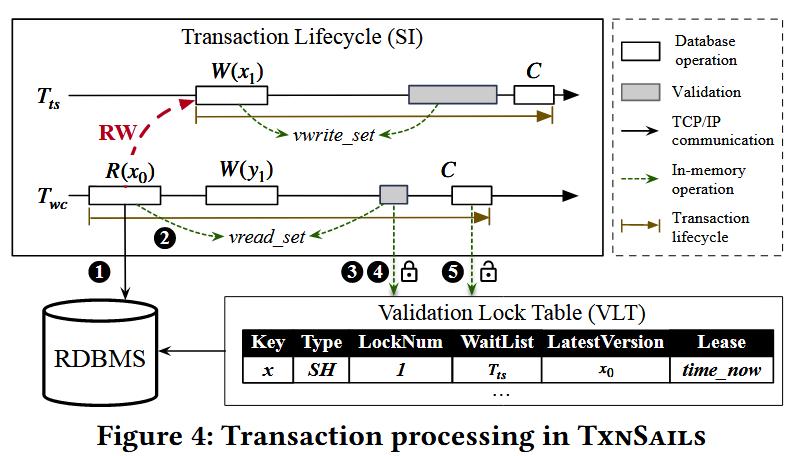
\includegraphics[width=0.98\linewidth]{figs/TxnSails-txn-proc}
		\end{column}
	\end{columns}
\end{frame}
%%%%%%%%%%%%%%%%%%%%

%%%%%%%%%%%%%%%%%%%%
\begin{frame}{VLDB2025 TxnSails-Achieving Serializable Transaction Scheduling with Self-Adaptive Isolation Level Selection}
	\textbf{Contributions: }
	\begin{itemize}
		\item 面向动态工作负载的自适应隔离级别选择机制:将工作负载特征建模为依赖图,利用 GNN 学习低隔离级别的性能收益与维持 SER 的开销之间的权衡关系,并实时预测未来工作负载的最优隔离级别(RC, SI 或 SER)。
	\end{itemize}
	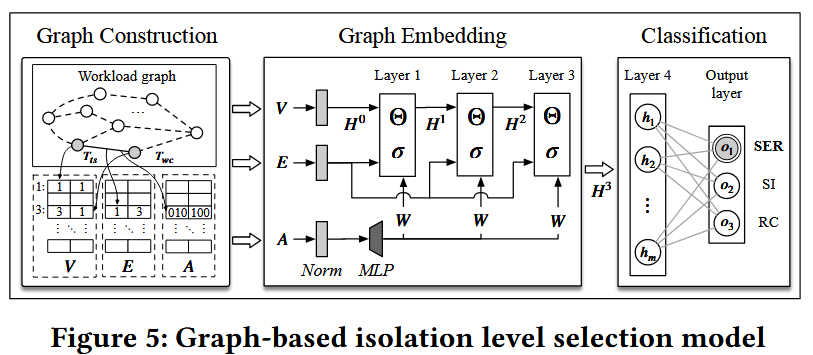
\includegraphics[width=0.8\linewidth]{figs/TxnSails-selection-model}
\end{frame}
%%%%%%%%%%%%%%%%%%%%

%%%%%%%%%%%%%%%%%%%%
\begin{frame}{VLDB2025 TxnSails-Achieving Serializable Transaction Scheduling with Self-Adaptive Isolation Level Selection}
	\begin{columns}
		\begin{column}{0.5\textwidth}
			\textbf{Contributions: }
			\begin{itemize}
				\item 跨隔离级别验证机制:当系统根据预测需要切换隔离级别时,检测可能出现的新的危险结构避免破坏 SER;并通过确保提交顺序与依赖顺序一致(必要时中止事务)来保证切换过程中的可串行化,且避免了长时间的阻塞或高中止率。
			\end{itemize}
		\end{column}
		\begin{column}{0.5\textwidth}
			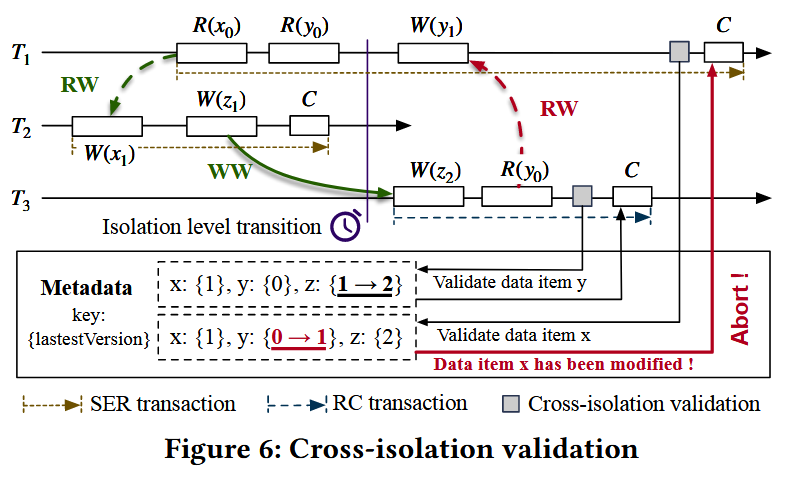
\includegraphics[width=0.98\linewidth]{figs/TxnSails-cross-isolation}
		\end{column}
	\end{columns}
\end{frame}
%%%%%%%%%%%%%%%%%%%%